\documentclass{article}
\usepackage[utf8]{inputenc}
\usepackage{subfigure}
\usepackage{geometry}
\usepackage{siunitx}

\geometry{
 a4paper,
 total={160mm,247mm},
 left=25mm,
 top=25mm,
 }

\title{Comp Astro Assignment 1}
\author{Cameron Smith }
\usepackage{natbib}
\usepackage{graphicx}

\begin{document}

\maketitle

\section*{Part 1}



\section*{Part 2}
\subsection*{a)}

\begin{figure}[h]
    \centering
    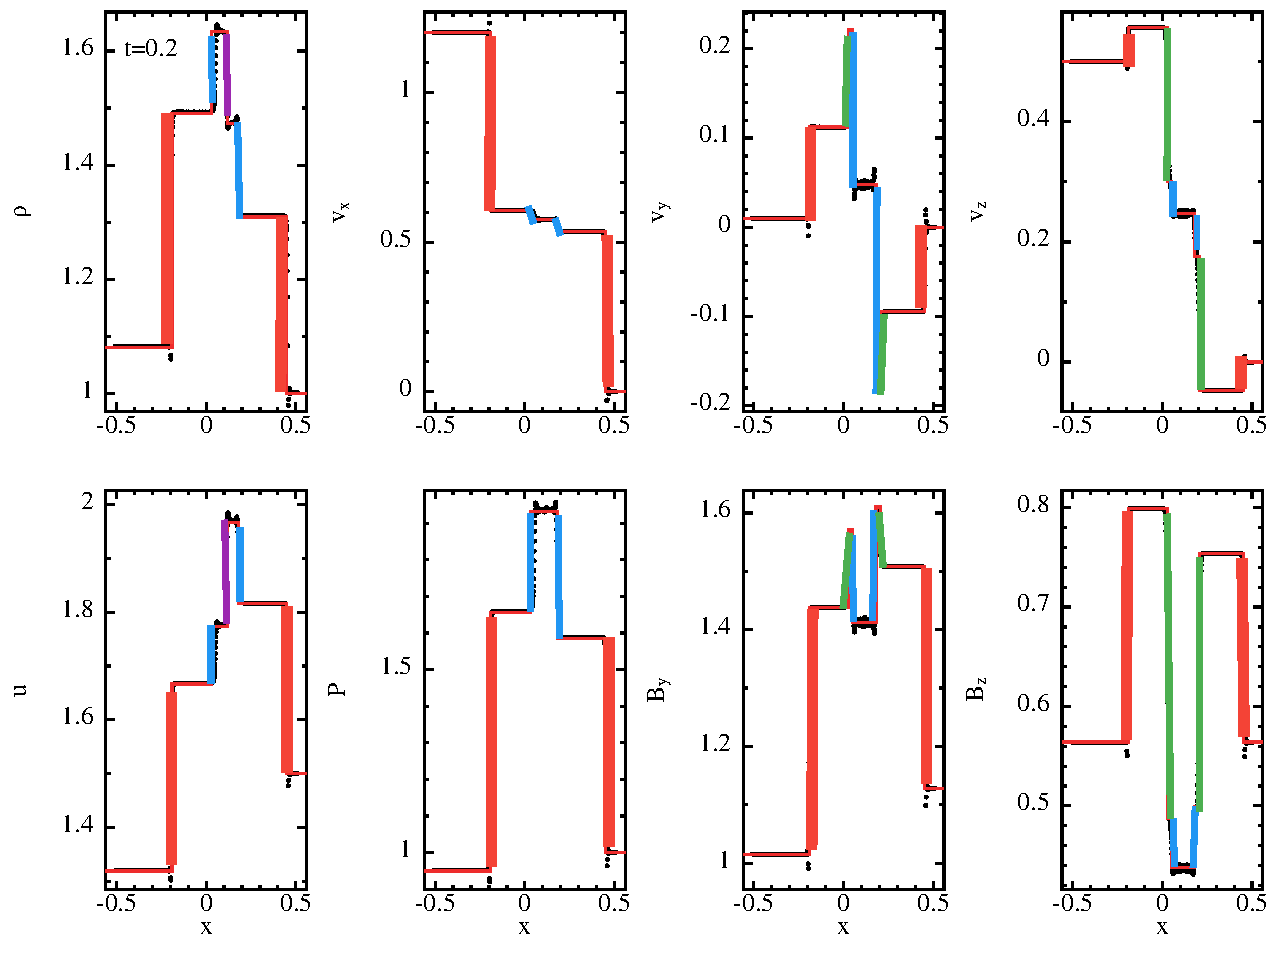
\includegraphics[width=\linewidth]{2a_labeled.pdf}
    \caption{``1.75D'' magnetised shock tube. Red Corresponds to a fast wave,
    blue corresponds to a slow wave, green corresponds to an alfven wave, and
    purple corresponds to a contact discontinuity.
    }
    \label{2a}
\end{figure}

\subsection*{b)}
\begin{figure}[h]
    \centering
    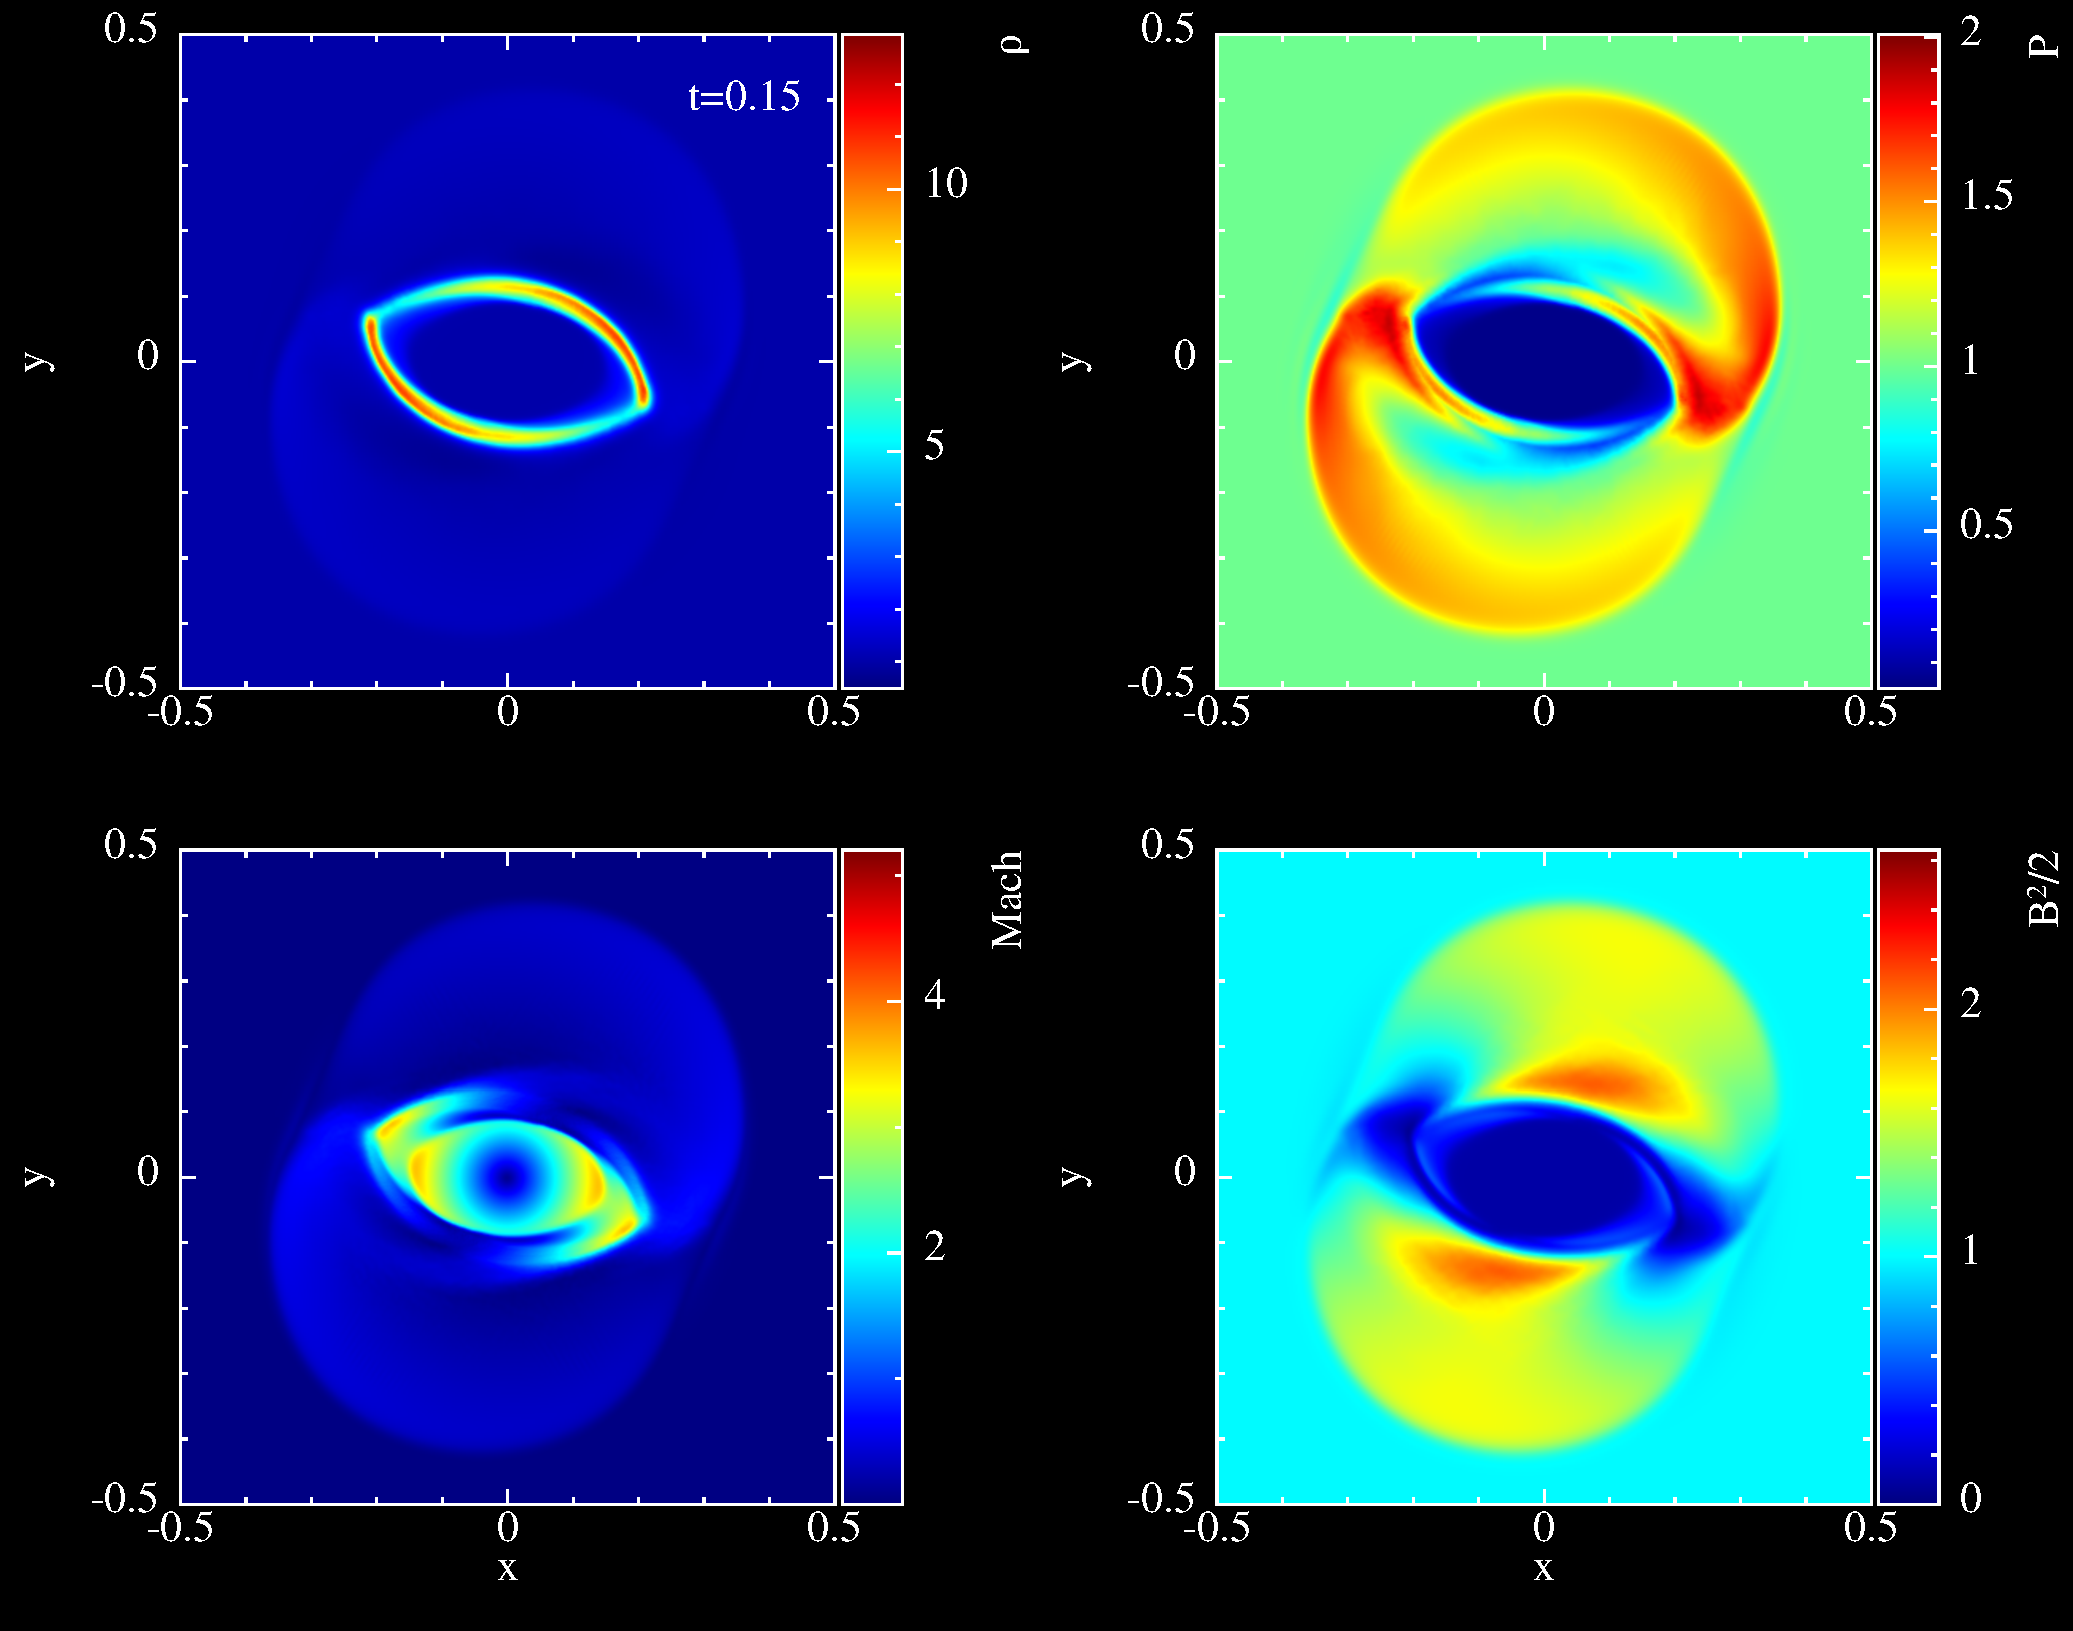
\includegraphics[width=\linewidth]{2b.pdf}
    \caption{}
    \label{2b}
\end{figure}

\section*{Part 3}
\subsection*{a)}

\begin{figure}%
    \centering
    \subfigure[]{%
    \label{fig:one_fluid}%
    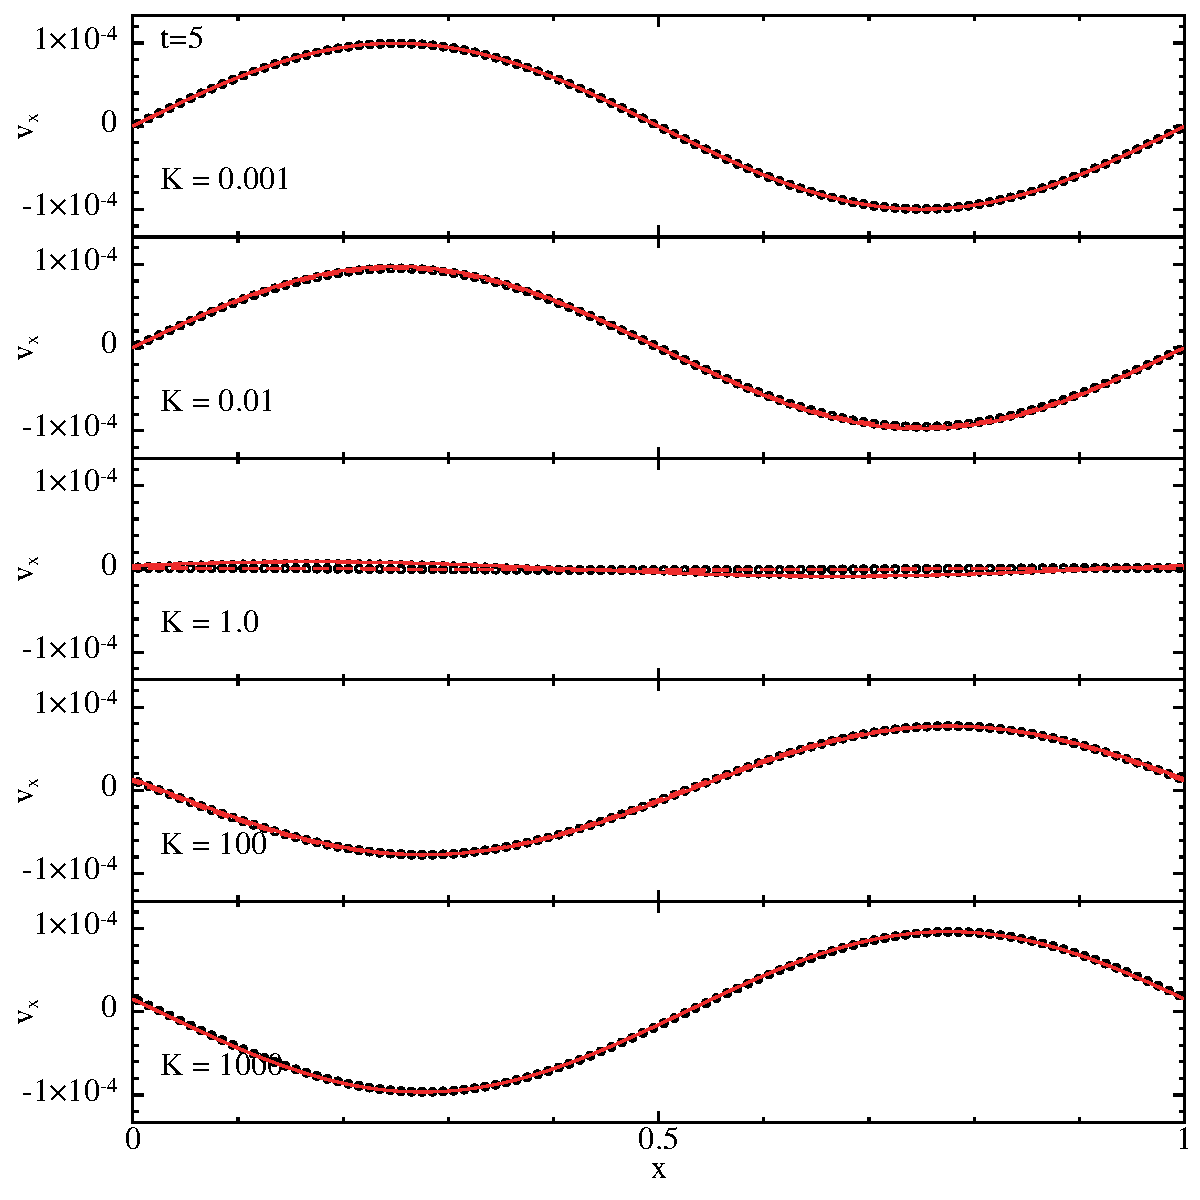
\includegraphics[height=3in]{one_fluid.pdf}}%
    \qquad
    \subfigure[]{%
    \label{fig:two_fluid}%
    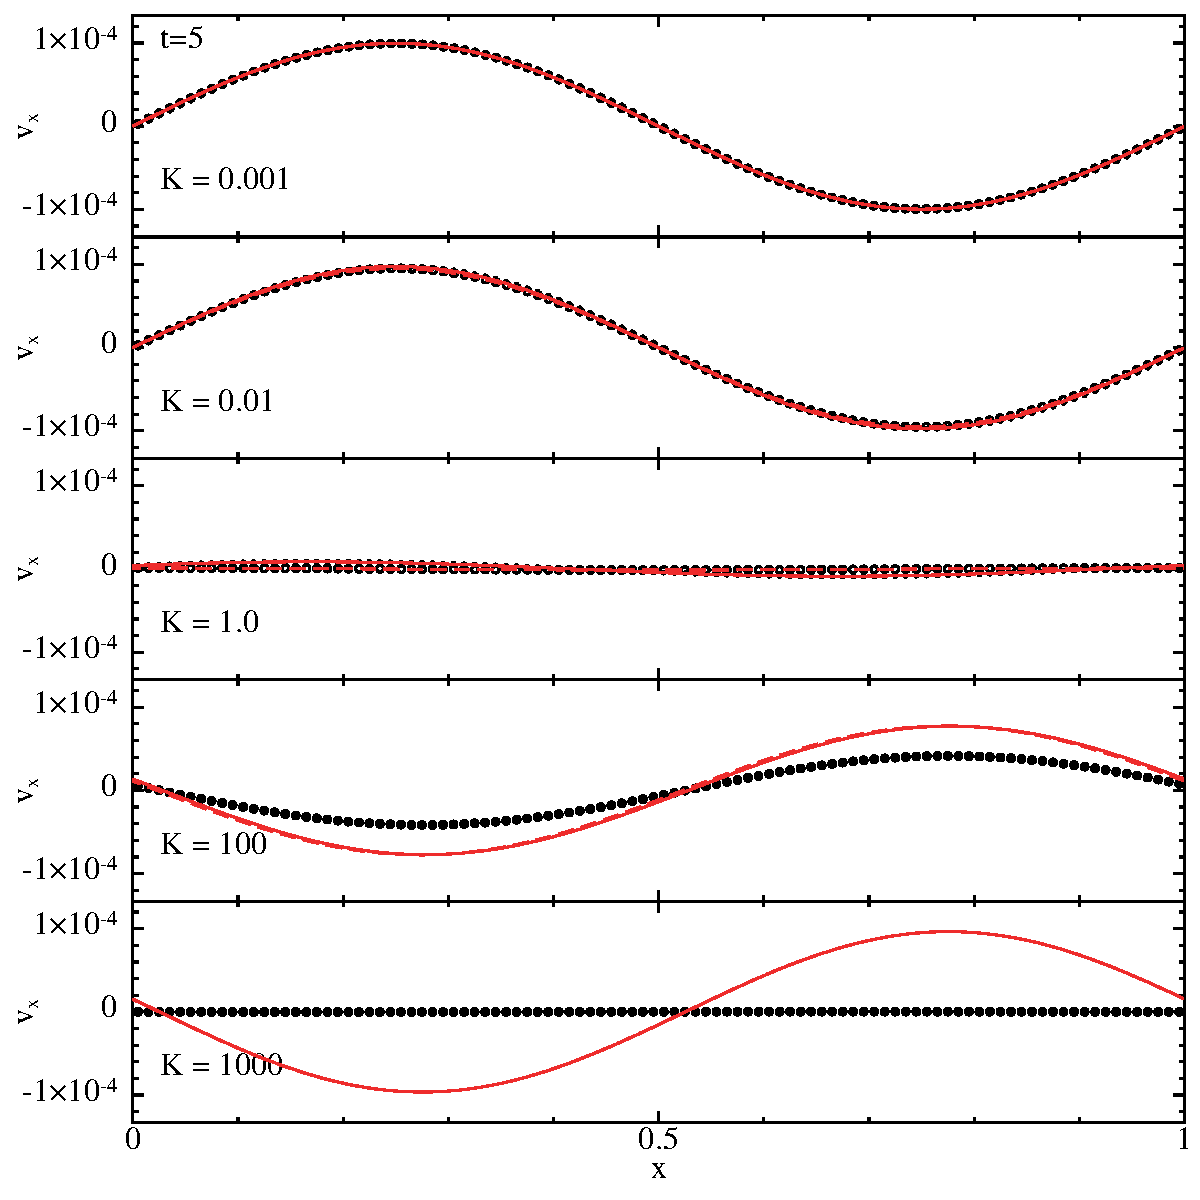
\includegraphics[height=3in]{two_fluid.pdf}}%
    \caption[]{\subref{fig:one_fluid} One fluid. \subref{fig:two_fluid} Two fluid.}
    \end{figure}
    


\end{document}
